\section{Exercises}

%____________________
\subsection{Estimating unknown parameters}

% 1

\eoce{\qt{Identify the parameter, Part I} For each of the following situations, state whether the parameter of interest is a mean or a proportion. It may be helpful to examine whether individual responses are numerical or categorical.
\begin{parts}
\item In a survey, one hundred college students are asked how many hours per week they spend on the Internet.
\item In a survey, one hundred college students are asked: ``What percentage of the time you spend on the Internet is part of your course work?"
\item In a survey, one hundred college students are asked whether or not they cited information from Wikipedia in their papers.
\item In a survey, one hundred college students are asked what percentage of their total weekly spending is on alcoholic beverages.
\item In a sample of one hundred recent college graduates, it is found that 85 percent expect to get a job within one year of their graduation date.
\end{parts}
}{}

% 2

\eoce{\qt{Identify the parameter, Part II} For each of the following situations, state whether the parameter of interest is a mean or a proportion. 
\begin{parts}
\item A poll shows that 64\% of Americans personally worry a great deal about federal spending and the budget deficit.
\item A survey reports that local TV news has shown a 17\% increase in revenue between 2009 and 2011 while newspaper revenues decreased by 6.4\% during this time period.
\item In a survey, high school and college students are asked whether or not they use geolocation services on their smart phones.
\item In a survey, internet users are asked whether or not they purchased any Groupon coupons.
\item In a survey, internet users are asked how many Groupon coupons they purchased over the last year.
\end{parts}
}{}

% 3

\eoce{\qt{College credits} \label{credits} A college counselor is interested in estimating how many credits a student typically enrolls in each semester. The counselor decides to randomly sample 100 students by using the registrar's database of students. The histogram below shows the distribution of the number of credits taken by these students. Sample statistics for this distribution are also provided.\\
\begin{minipage}[c]{0.75\textwidth}
\begin{center}
\includegraphics[width=\textwidth]{ch_distributions/figures/eoce/credits/credits}
\end{center}
\end{minipage}
\begin{minipage}[c]{0.22\textwidth}
\begin{center}
\begin{tabular}{l|r l}
Min		& 8 \\
Q1		& 13 \\
Median	& 14 \\
Mean	& 13.65 \\
SD		& 1.91 \\
Q3		& 15 \\
Max		& 18 \\
\end{tabular}
\end{center}
\end{minipage}
\begin{parts}
\item What is the point estimate for the average number of credits taken per semester by students at this college? What about the median?
\item What is the point estimate for the standard deviation of the number of credits taken per semester by students at this college? What about the IQR? \textA{\textbf{(See the next page for parts~(c)-(e).)}}
\item Is a load of 16 credits unusually high for this college? What about 18 credits? Explain your reasoning. \textit{Hint:} Observations farther than two standard deviations from the mean are usually considered to be unusual.
\item The college counselor takes another random sample of 100 students and this time finds a sample mean of 14.02 units. Should she be surprised that this sample statistic is slightly different than the one from the original sample? Explain your reasoning.
\item The sample means given above are point estimates for the mean number of credits taken by all students at that college. What measures do we use to quantify the variability of this estimate (Hint: recall that $SD_{\bar{x}}=\frac{\sigma}{\sqrt{n}}$)? Compute this quantity using the data from the original sample.\end{parts}
}{}

% 4

\eoce{\qt{Heights of adults} \label{heights} Researchers studying anthropometry collected body girth measurements and skeletal diameter measurements, as well as age, weight, height and gender, for 507 physically active individuals. The histogram below shows the sample distribution of heights in centimeters. \footfullcite{Heinz:2003} \\
\begin{minipage}[c]{0.75\textwidth}
\begin{center}
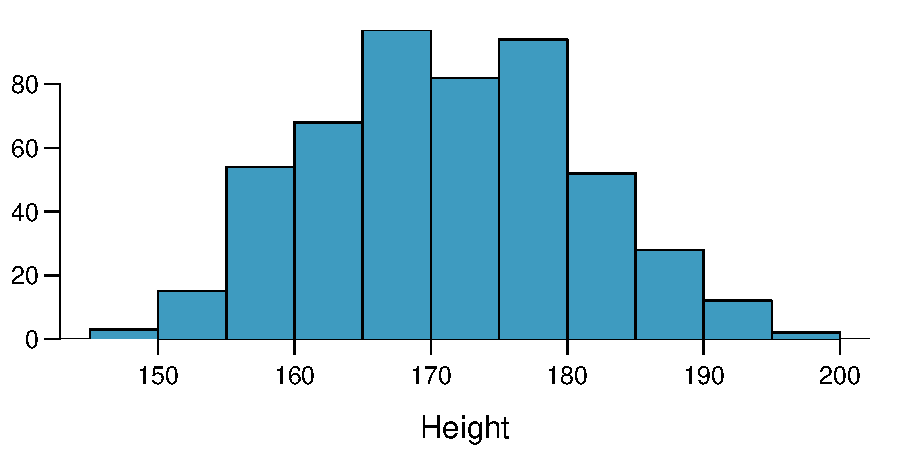
\includegraphics[width=\textwidth]{ch_distributions/figures/eoce/bdims/bdims_heights}
\end{center}
\end{minipage}
\begin{minipage}[c]{0.23\textwidth}
\begin{center}
\begin{tabular}{l|r l}
Min		& 147.2 \\
Q1		& 163.8 \\
Median	& 170.3 \\
Mean	& 171.1 \\
SD		&  9.4 \\
Q3		& 177.8 \\
Max		& 198.1 \\
\end{tabular}
\end{center}
\end{minipage}
\begin{parts}
\item What is the point estimate for the average height of active individuals? What about the median?
\item What is the point estimate for the standard deviation of the heights of active individuals? What about the IQR?
\item Is a person who is 1m 80cm (180 cm) tall considered unusually tall? And is a person who is 1m 55cm (155cm) considered unusually short? Explain your reasoning.
\item The researchers take another random sample of physically active individuals. Would you expect the mean and the standard deviation of this new sample to be the ones given above? Explain your reasoning.
\item The sample means obtained are point estimates for the mean height of all active individuals, if the sample of individuals is equivalent to a simple random sample. What measure do we use to quantify the variability of such an estimate (Hint: recall that $SD_{\bar{x}}=\frac{\sigma}{\sqrt{n}}$)? Compute this quantity using the data from the original sample under the condition that the data are a simple random sample. 
\end{parts}
}{}

\textA{\newpage}

% 5

\eoce{\qt{Hen eggs} The distribution of the number of eggs laid by a certain species of hen during their breeding period has a mean of 35 eggs with a standard deviation of 18.2. Suppose a group of researchers randomly samples 45 hens of this species, counts the number of eggs laid during their breeding period, and records the sample mean. They repeat this 1,000 times, and build a distribution of sample means. 
\begin{parts}
\item What is this distribution called? 
\item Would you expect the shape of this distribution to be symmetric, right skewed, or left skewed? Explain your reasoning.
\item Calculate the variability of this distribution and state the appropriate term used to refer to this value.
\item Suppose the researchers' budget is reduced and they are only able to collect random samples of 10 hens. The sample mean of the number of eggs is recorded, and we repeat this 1,000 times, and build a new distribution of sample means. How will the variability of this new distribution compare to the variability of the original distribution?
\end{parts}
}{}

% 6

\eoce{\qt{Art after school} Elijah and Tyler, two high school juniors, conducted a survey on 15 students at their school, asking the students whether they would like the school to offer an after-school art program, counted the number of ``yes" answers, and recorded the sample proportion. 14 out of the 15 students responded ``yes". They repeated this 100 times and built a distribution of sample means. 
\begin{parts}
\item What is this distribution called? 
\item Would you expect the shape of this distribution to be symmetric, right skewed, or left skewed? Explain your reasoning.
\item Calculate the variability of this distribution and state the appropriate term used to refer to this value.
\item Suppose that the students were able to recruit a few more friends to help them with sampling, and are now able to collect data from random samples of 25 students. Once again, they record the number of ``yes" answers, and record the sample proportion, and repeat this 100 times to build a new distribution of sample proportions. How will the variability of this new distribution compare to the variability of the original distribution?
\end{parts}
}{}

%_________________
\subsection{Confidence intervals}

% 7

\eoce{\qt{Chronic illness, Part I} \label{ChronicIllnessP1}
In 2013, the Pew Research Foundation reported that ``45\% of U.S. adults report that they live with one or more chronic conditions''.\footfullcite{data:pewdiagnosis:2013} However, this value was based on a sample, so it may not be a perfect estimate for the population parameter of interest on its own. The study reported a standard error of about 1.2\%, and a normal model may reasonably be used in this setting. Create a 95\% confidence interval for the proportion of U.S. adults who live with one or more chronic conditions. Also interpret the confidence interval in the context of the study.
}{}

% 8

\eoce{\qt{Twitter users and news, Part I} A poll conducted in 2013 found that 52\% of U.S. adult Twitter users get at least some news on Twitter.\footfullcite{data:pewtwitternews:2013}. The standard error for this estimate was 2.4\%, and a normal distribution may be used to model the sample proportion. Construct a 99\% confidence interval for the fraction of U.S. adult Twitter users who get some news on Twitter, and interpret the confidence interval in context.
}{}

\textA{\pagebreak}

% 9

\eoce{\qt{Chronic illness, Part II} In 2013, the Pew Research Foundation reported that ``45\% of U.S. adults report that they live with one or more chronic conditions'', and the standard error for this estimate is 1.2\%.
Identify each of the following statements as true or false. Provide an explanation to justify each of your answers.
\begin{parts}
\item We can say with certainty that the confidence interval from Exerise~\ref{ChronicIllnessP1} contains the true percentage of U.S. adults who suffer from a chronic illness.
\item If we repeated this study 1,000 times and constructed a 95\% confidence interval for each study, then approximately 950 of those confidence intervals would contain the true fraction of U.S. adults who suffer from chronic illnesses.
\item The poll provides statistically significant evidence (at the $\alpha = 0.05$ level) that the percentage of U.S. adults who suffer from chronic illnesses is below 50\%.
\item Since the standard error is 1.2\%, only 1.2\% of people in the study communicated uncertainty about their answer.
\end{parts}
}{}

% 10

\eoce{\qt{Twitter users and news, Part II} A poll conducted in 2013 found that 52\% of U.S. adult Twitter users get at least some news on Twitter, and the standard error for this estimate was 2.4\%. Identify each of the following statements as true or false. Provide an explanation to justify each of your answers.
\begin{parts}
\item The data provide statistically significant evidence that more than half of U.S. adult Twitter users get some news through Twitter. Use a significance level of $\alpha = 0.01$.
\item Since the standard error is 2.4\%, we can conclude that 97.6\% of all U.S. adult Twitter users were included in the study.
\item If we want to reduce the standard error of the estimate, we should collect less data.
\item If we construct a 90\% confidence interval for the percentage of U.S. adults Twitter users who get some news through Twitter, this confidence interval will be wider than a corresponding 99\% confidence interval.
\end{parts}
}{}

% 11

\eoce{\qt{Relaxing after work} The 2010 General Social Survey asked the question: ``After an average work day, about how many hours do you have to relax or pursue activities that you enjoy?" to a random sample of 1,155 Americans.\footfullcite{data:gss:2010} A 95\% confidence interval for the mean number of hours spent relaxing or pursuing activities they enjoy was (1.38, 1.92).
\begin{parts}
\item Interpret this interval in context of the data.
\item Suppose another set of researchers reported a confidence interval with a larger margin of error based on the same sample of 1,155 Americans. How does their confidence level compare to the confidence level of the interval stated above?
\item Suppose next year a new survey asking the same question is conducted, and this time the sample size is 2,500. Assuming that the population characteristics, with respect to how much time people spend relaxing after work, have not changed much within a year. How will the margin of error of the 95\% confidence interval constructed based on data from the new survey compare to the margin of error of the interval stated above?
\end{parts}
}{}

\textA{\pagebreak}

% 12

\eoce{\qt{Take a walk} The Centers for Disease Control monitors the physical activity level of Americans. A recent survey on a random sample of 23,129 Americans yielded a 95\% confidence interval of 61.1\% to 62.9\% for the proportion of Americans who walk for at least 10 minutes per day.
\begin{parts}
\item Interpret this interval in context of the data.
\item Suppose another set of researchers reported a confidence interval with a larger margin of error based on the same sample of 23,129 Americans. How does their confidence level compare to the confidence level of the interval stated above?
\item Suppose next year a new survey asking the same question is conducted, and this time the sample size is 10,000. Assuming that the population characteristics, with respect to walking habits, have not changed much within a year, how will the width of the confidence interval constructed based on data from the new survey compare to the width of the interval stated above?
\end{parts}
}{}

% 13

\eoce{\qt{Women leaders, Part I} \label{womenLeaders} A November 2014 Pew Research poll on women and leadership asked respondents what they believed is holding women back from top jobs. 43\% of the respondents said that women are held to higher standards than men when being considered for top executive business positions. This result is based on 1,835 randomly sampled national adults. \footfullcite{data:pewwomenleaders:2014}
\begin{parts}
\item Construct a 95\% confidence interval for the proportion of Americans who believe women are held to higher standards than men when being considered for top executive business positions. 
\item How would you expect the width of a 90\% confidence interval to compare to the interval you calculated in part (a)? Explain your reasoning.
\item Now construct the 90\% confidence interval, and comment on whether your answer to part (b) is confirmed.
\end{parts}
}{}

% 14

\eoce{\qt{Women leaders, Part II}  The poll introduced in Exercise~\ref{womenLeaders} also asked whether respondents expected to see a female president in their lifetime. 78\% of the 1,835 respondents said ``yes".
\begin{parts}
\item Construct a 90\% confidence interval for the proportion of Americans who expect to see a female president in their lifetime, and interpret this interval in context of the data.
\item How would you expect the width of a 98\% confidence interval to compare to the interval you calculated in part (a)? Explain your reasoning.
\item Now construct the 98\% confidence interval, and comment on whether your answer to part (b) is confirmed.
\end{parts}
}{}


\textA{\newpage}

%_________________
\subsection{Introducing hypothesis testing}

% 15

\eoce{\qt{Social experiment, Part I} \label{socExpP1} A ``social experiment" conducted by a TV program questioned what people do when they see a very obviously bruised woman getting picked on by her boyfriend. On two different occasions at the same restaurant, the same couple was depicted. In one scenario the woman was dressed ``provocatively'' and in the other scenario the woman was dressed ``conservatively''. The table below shows how many restaurant diners were present under each scenario, and whether or not they intervened.
\begin{center}
\begin{tabular}{ll cc c} 
			&				& \multicolumn{2}{c}{\textit{Scenario}} \\
\cline{3-4}
							&			& Provocative	& Conservative 	& Total	\\
\cline{2-5}
\multirow{2}{*}{\textit{Intervene}}	&Yes 		& 5	 	& 15		& 20 	\\
							&No			& 15	 	& 10 	 	& 25 \\
\cline{2-5}
							&Total		& 20		& 25		& 45 \\
\end{tabular}
\end{center}
A simulation was conducted to test if people react differently under the two scenarios. 10,000 simulated differences were generated to construct the null distribution shown. The value $\hat{p}_{pr, sim}$ represents the proportion of diners who intervened in the simulation for the provocatively dressed woman, and $\hat{p}_{con, sim}$ is the proportion for the conservatively dressed woman.
\begin{center}
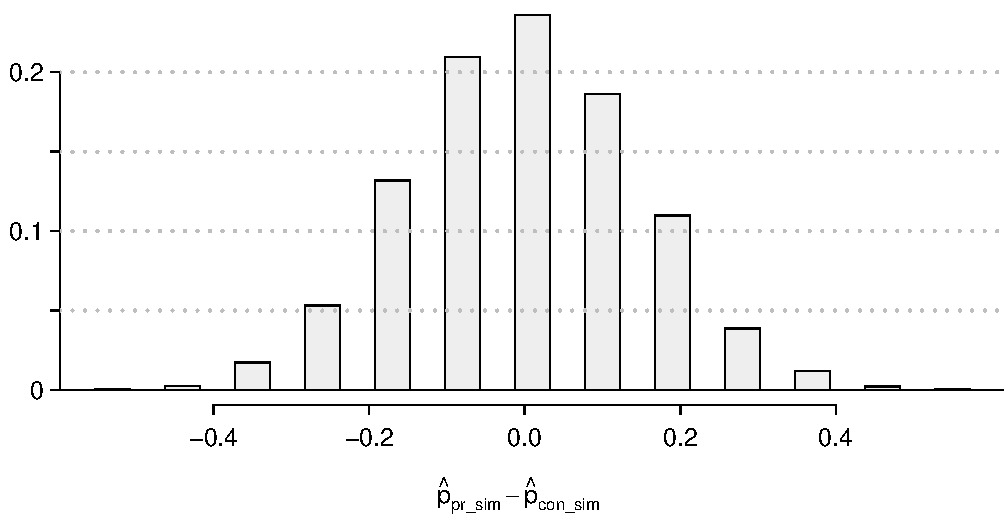
\includegraphics[width=0.9\textwidth]{ch_inference_for_props/figures/eoce/socExp/socExp}
\end{center}
\begin{parts}
\item What are the hypotheses? For the purposes of this exercise, you may assume that each observed person at the restaurant behaved independently, though we would want to evaluate this assumption more rigorously if we were reporting these results.
\item Calculate the observed difference between the rates of intervention under the provocative and conservative scenarios: $\hat{p}_{pr} - \hat{p}_{con}$.
\item Estimate the p-value using the figure above and determine the conclusion of the hypothesis test.
\end{parts}
}{}

\textA{\newpage}

% 16

\eoce{\qt{Is yawning contagious, Part I} \label{yawningContageousP1} An experiment conducted by the \textit{MythBusters}, a science entertainment TV program on the Discovery Channel, tested if a person can be subconsciously influenced into yawning if another person near them yawns. 50 people were randomly assigned to two groups: 34 to a group where a person near them yawned (treatment) and 16 to a group where there wasn't a person yawning near them (control). The following table shows the results of this experiment. \footfullcite{data:yawn}
\begin{center}
\begin{tabular}{ll cc c} 
			&				& \multicolumn{2}{c}{\textit{Group}} \\
\cline{3-4}
							&			& Treatment	& Control 	& Total	\\
\cline{2-5}
\multirow{2}{*}{\textit{Result}}		&Yawn 		& 10	 	& 4		& 14 	\\
							&Not Yawn	& 24	 	& 12 	 	& 36 \\
\cline{2-5}
							&Total		& 34		& 16		& 50 \\
\end{tabular}
\end{center}
A simulation was conducted to understand the distribution of the test statistic under the assumption of independence: having someone yawn near another person has no influence on if the other person will yawn. In order to conduct the simulation, a researcher wrote yawn on 14 index cards and not yawn on 36 index cards to indicate whether or not a person yawned. Then he shuffled the cards and dealt them into two groups of size 34 and 16 for treatment and control, respectively. He counted how many participants in each simulated group yawned in an apparent response to a nearby yawning person, and calculated the difference between the simulated proportions of yawning as $\hat{p}_{trtmt,sim} - \hat{p}_{ctrl,sim}$. This simulation was repeated 10,000 times using software to obtain 10,000 differences that are due to chance alone. The histogram shows the distribution of the simulated differences.
\begin{center}
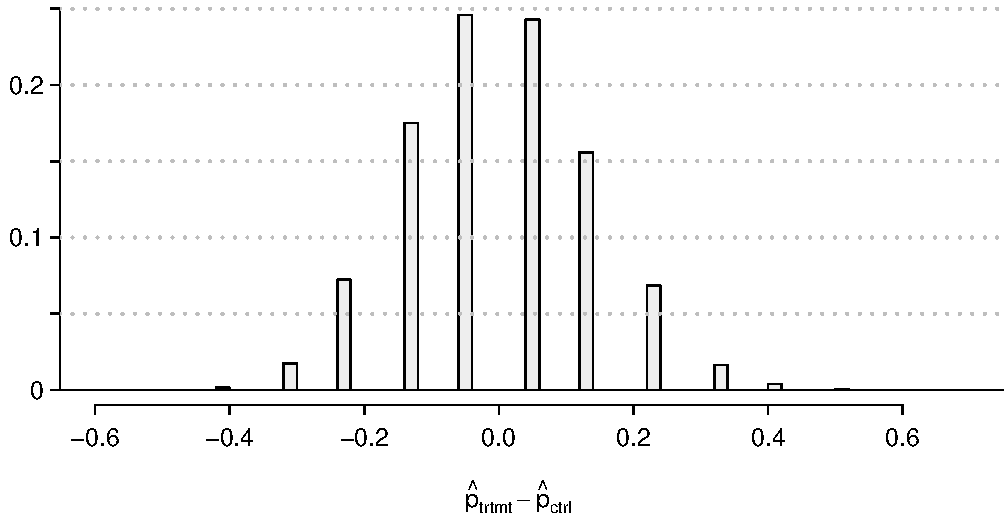
\includegraphics[width=0.9\textwidth]{ch_inference_for_props/figures/eoce/yawn/yawn}
\end{center}
\begin{parts}
\item What are the hypotheses?
\item Calculate the observed difference between the yawning rates under the two scenarios.
\item Estimate the p-value using the figure above and determine the conclusion of the hypothesis test.
\end{parts}
}{}

% 17

\eoce{\qt{Social experiment, Part II} In Exercise~\ref{socExpP1}, we encountered a scenario where researchers were evaluating the impact of the way someone is dressed against the actions of people around them. In that exercise, researchers may have believed that dressing provocatively may reduce the chance of bystander intervention. One might be tempted to use a one-sided hypothesis test for this study. Discuss the drawbacks of doing so in 1-3 sentences.
}{}

% 18

\eoce{\qt{Is yawning contagious, Part II} Exercise~\ref{yawningContageousP1} describes an experiment by Myth Busters, where they examined whether a person yawning would affect whether others to yawn. The traditional belief is that yawning is contagious -- one yawn can lead to another yawn, which might lead to another, and so on. In that exercise, there was the option of selecting a one-sided or two-sided test. Which would you recommend (or which did you choose)? Justify your answer in 1-3 sentences.
}{}

% 19

\eoce{\qt{The Egyptian Revolution} \label{EgyptianRevolutionEOCE} A popular uprising that started on January 25, 2011 in Egypt led to the 2011 Egyptian Revolution. Polls show that about 69\% of American adults followed the news about the political crisis and demonstrations in Egypt closely during the first couple weeks following the start of the uprising. Among a random sample of 30 high school students, it was found that only 17 of them followed the news about Egypt closely during this time. \footfullcite{data:egypt}
\begin{parts}
\item Write the hypotheses for testing if the proportion of high school students who followed the news about Egypt is different than the proportion of American adults who did.
\item Calculate the proportion of high schoolers in this sample who followed the news about Egypt closely during this time.
\item Describe how to perform a simulation and, once you had results, how to estimate the p-value.
\item Below is a histogram showing the distribution of $\hat{p}_{sim}$ in 10,000 simulations under the null hypothesis. Estimate the p-value using the plot and determine the conclusion of the hypothesis test.
\begin{center}
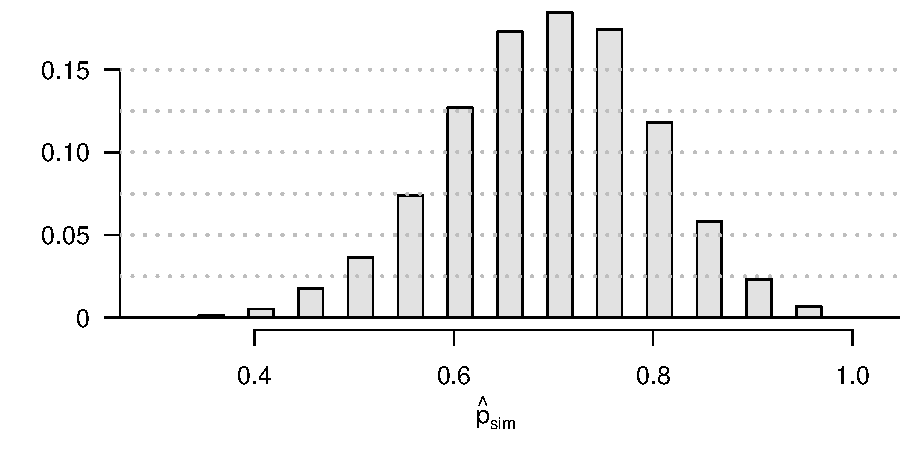
\includegraphics[width=0.85\textwidth]{ch_inference_for_props/figures/eoce/egypt/egypt}
\end{center}
\end{parts}
}{}

\textA{\newpage}

% 20

\eoce{\qt{Assisted Reproduction} \label{AssistedReproductionEOCE} Assisted Reproductive Technology (ART) is a collection of techniques that help facilitate pregnancy (e.g. in vitro fertilization). A 2008 report by the Centers for Disease Control and Prevention estimated that ART has been successful in leading to a live birth in 31\% of cases \footfullcite{web:art}. A new fertility clinic claims that their success rate is higher than average. A random sample of 30 of their patients yielded a success rate of 40\%. A consumer watchdog group would like to determine if this provides strong evidence to support the company's claim.
\begin{parts}
\item Write the hypotheses to test if the success rate for ART at this clinic is significantly higher than the success rate reported by the CDC.
\item Describe a setup for a simulation that would be appropriate in this situation and how the p-value can be calculated using the simulation results.
\item Below is a histogram showing the distribution of $\hat{p}_{sim}$ in 10,000 simulations under the null hypothesis. Estimate the p-value using the plot and use it to evaluate the hypotheses.
\item After performing this analysis, the consumer group releases the following news headline: ``Infertility clinic falsely advertises better success rates". Comment on the appropriateness of this statement.
\begin{center}
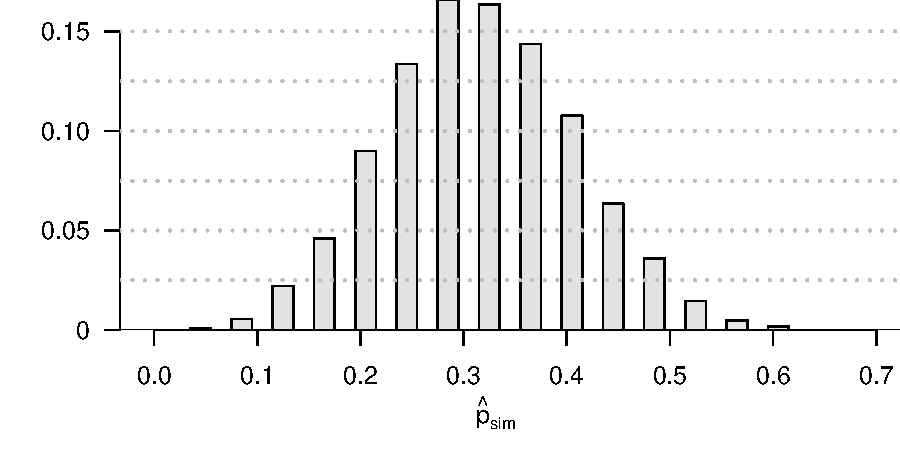
\includegraphics[width=0.85\textwidth]{ch_inference_for_props/figures/eoce/art/art}
\end{center}
\end{parts}
}{}

% 21

\eoce{\qt{Spam mail, Part I} \label{spam} The 2004 National Technology Readiness Survey sponsored by the Smith School of Business at the University of Maryland surveyed 418 randomly sampled Americans, asking them how many spam emails they receive per day. The survey was repeated on a new random sample of 499 Americans in 2009.\footfullcite{webpage:spam}
\begin{parts}
\item What are the hypotheses for evaluating if the average spam emails per day has changed from 2004 to 2009.
\item In 2004 the mean was 18.5 spam emails per day, and in 2009 this value was 14.9 emails per day. What is the point estimate for the difference between the two population means?
\item A report on the survey states that the observed difference between the sample means is not statistically significant. Explain what this means in context of the hypothesis test and data.
\item Would you expect a confidence interval for the difference between the two population means to contain 0? Explain your reasoning.
\end{parts}
}{}

\textA{\pagebreak}

% 22

\eoce{\qt{Nearsightedness} It is believed that nearsightedness affects about 8\% of all children. In a random sample of 194 children, 21 are nearsighted.
\begin{parts}
\item Construct hypotheses appropriate for the following question: do these data provide evidence that the 8\% value is inaccurate?
\item What proportion of children in this sample are nearsighted?
\item Given that the standard error of the sample proportion is 0.0195 and the point estimate follows a nearly normal distribution, calculate the test statistic (the Z-statistic).
\item What is the p-value for this hypothesis test?
\item What is the conclusion of the hypothesis test?
\end{parts}
}{}

% 23

\eoce{\qt{Spam mail, Part II} The National Technology Readiness Survey from Exercise~\ref{spam} also asked Americans how often they delete spam emails. 23\% of the respondents in 2004 said they delete their spam mail once a month or less, and in 2009 this value was 16\%.
\begin{parts}
\item What are the hypotheses for evaluating if the proportion of those who delete their email once a month or less has changed from 2004 to 2009?
\item What is the point estimate for the difference between the two population proportions?
\item A report on the survey states that the observed decrease from 2004 to 2009 is statistically significant. Explain what this means in context of the hypothesis test and the data.
\item Would you expect a confidence interval for the difference between the two population proportions to contain 0? Explain your reasoning.
\end{parts}
}{}

% 24

\eoce{\qt{Unemployment and relationship problems} A USA Today/Gallup poll conducted between 2010 and 2011 asked a group of unemployed and underemployed Americans if they have had major problems in their relationships with their spouse or another close family member as a result of not having a job (if unemployed) or not having a full-time job (if underemployed). 27\% of the 1,145 unemployed respondents and 25\% of the 675 underemployed respondents said they had major problems in relationships as a result of their employment status.
\begin{parts}
\item What are the hypotheses for evaluating if the proportions of unemployed and underemployed people who had relationship problems were different?
\item The p-value for this hypothesis test is approximately 0.35. Explain what this means in context of the hypothesis test and the data.
\end{parts}
}{}

%25

\eoce{\qt{Testing for Fibromyalgia} A patient named Diana was diagnosed with Fibromyalgia, a long-term syndrome of body pain, and was prescribed anti-depressants. Being the skeptic that she is, Diana didn't initially believe that anti-depressants would help her symptoms. However after a couple months of being on the medication she decides that the anti-depressants are working, because she feels like her symptoms are in fact getting better.
\begin{parts}
\item Write the hypotheses in words for Diana's skeptical position when she started taking the anti-depressants.
\item What is a Type~I Error in this context?
\item What is a Type~II Error in this context?
\end{parts}
}{}

\textA{\newpage}

% 26

\eoce{\qt{Testing for food safety} A food safety inspector is called upon to investigate a restaurant with a few customer reports of poor sanitation practices. The food safety inspector uses a hypothesis testing framework to evaluate whether regulations are not being met. If he decides the restaurant is in gross violation, its license to serve food will be revoked.
\begin{parts}
\item Write the hypotheses in words.
\item What is a Type~I Error in this context?
\item What is a Type~II Error in this context?
\item Which error is more problematic for the restaurant owner? Why?
\item Which error is more problematic for the diners? Why?
\item As a diner, would you prefer that the food safety inspector requires strong evidence or very strong evidence of health concerns before revoking a restaurant's license? Explain your reasoning.
\end{parts}
}{}

% 27

\eoce{\qt{True / False} Determine whether the following statement is true or false, and explain your reasoning: ``A cutoff of $\alpha$ = 0.05 is the ideal value for all hypothesis tests."
}{}

% 28

\eoce{\qt{True / False} Determine whether the following statement is true or false, and explain your reasoning: ``Power of a test and the probability of making a Type~I Error are complements."
}{}

% 29

\eoce{\qtq{Which is higher} In each part below, there is a value of interest and two scenarios (I and II). For each part, report if the value of interest is larger under scenario I, scenario II, or whether the value is equal under the scenarios.
\begin{parts}
\item The standard error of $\bar{x}$ when $s = 120$ and (I) n = 25 or (II) n = 125.
\item The margin of error of a confidence interval when the confidence level is (I) 90\% or (II) 80\%.
\item The p-value for a Z-statistic of 2.5 when (I) n = 500 or (II) n = 1000.
\item The probability of making a Type~II Error when the alternative hypothesis is true and the significance level is (I) 0.05 or (II) 0.10.
\end{parts}
}{}

% 30

\eoce{\qt{True or false} Determine if the following statements are true or false, and explain your reasoning. If false, state how it could be corrected.
\begin{parts}
\item If a given value (for example, the null hypothesized value of a parameter) is within a 95\% confidence interval, it will also be within a 99\% confidence interval.
\item Decreasing the significance level ($\alpha$) will increase the probability of making a Type~I Error.
\item Suppose the null hypothesis is $\mu = 5$ and we fail to reject $H_0$. Under this scenario, the true population mean is 5.
\item If the alternative hypothesis is true, then the probability of making a Type~II Error and the power of a test add up to 1.
\item With large sample sizes, even small differences between the null value and the true value of the parameter, a difference often called the effect size\index{effect size}, will be identified as statistically significant.
\end{parts}
}{}

%____________________
\subsection{Does it make sense?}

% 31
\eoce{\qt{True / False} Determine whether the following statement is true or false, and explain your reasoning: ``With large sample sizes, even small differences between the null value and the point estimate can be statistically significant."
}{}

% 32

\eoce{\qt{Same observation, different sample size} Suppose you conduct a hypothesis test based on a sample where the sample size is $n = 50$, and arrive at a p-value of 0.08. You then refer back to your notes and discover that you made a careless mistake, the sample size should have been $n = 500$. How, if at all, will your p-value change (increase or decrease)? Explain.
}{}